%!TEX TS-program = xelatex
% Исходная версия шаблона --- 
% https://www.writelatex.com/coursera/latex/5.1
\documentclass[c, dvipsnames]{beamer}  % [t], [c], или [b] --- вертикальное 
%\documentclass[handout, dvipsnames, c]{beamer} % Раздаточный материал (на слайдах всё сразу)
%выравнивание на слайдах (верх, центр, низ)
%\documentclass[handout, dvipsnames]{beamer} % Раздаточный материал (на слайдах всё сразу)
%\documentclass[aspectratio=169, dvipsnames]{beamer} % Соотношение сторон
\setbeamertemplate{navigation symbols}{}%remove navigation symbols

%\usetheme{Berkeley} % Тема оформленияLLL
%\usetheme{Bergen}
%\usetheme{CambridgeUS}
\usetheme{Boadilla}

\usecolortheme{crane} % Цветовая схема

%\useoutertheme{infolines} % Навигация 
%\useoutertheme{tree}
%\useoutertheme{miniframes}
%\useoutertheme{shadow}
%\useoutertheme{sidebar}
%\useoutertheme{smoothbars}
%\useoutertheme{smoothtree}
%\useoutertheme{split}
%\useoutertheme{default}


%\useinnertheme{circles}
\useinnertheme{rectangles}
%\useinnertheme{rounded}
%\useinnertheme{inmargin}


%%% Работа с русским языком
\usepackage[english,russian]{babel}   %% загружает пакет многоязыковой вёрстки
\usepackage{fontspec}      %% подготавливает загрузку шрифтов Open Type, True Type и др.
\defaultfontfeatures{Ligatures={TeX},Renderer=Basic}  %% свойства шрифтов по умолчанию
\setmainfont[Ligatures={TeX,Historic}]{Arial} %% задаёт основной шрифт документа
\setsansfont{Arial}                    %% задаёт шрифт без засечек
\setmonofont{Arial}
\usepackage{indentfirst}
\frenchspacing



%% Beamer по-русски
\newtheorem{rtheorem}{Теорема}
\newtheorem{rproof}{Доказательство}
\newtheorem{rexample}{Пример}

%%% Дополнительная работа с математикой
\usepackage{amsmath,amsfonts,amssymb,amsthm,mathtools} % AMS
\usepackage{icomma} % "Умная" запятая: $0,2$ --- число, $0, 2$ --- перечисление

%% Номера формул
\mathtoolsset{showonlyrefs=true} % Показывать номера только у тех формул, на которые есть \eqref{} в тексте.
%\usepackage{leqno} % Нумерация формул слева

%% Свои команды
\DeclareMathOperator{\sgn}{\mathop{sgn}}

%% Перенос знаков в формулах (по Львовскому)
\newcommand*{\hm}[1]{#1\nobreak\discretionary{}
{\hbox{$\mathsurround=0pt #1$}}{}}

%%% Работа с картинками
\usepackage{graphicx}  % Для вставки рисунков
\graphicspath{{images/}{images2/}}  % папки с картинками
\setlength\fboxsep{3pt} % Отступ рамки \fbox{} от рисунка
\setlength\fboxrule{1pt} % Толщина линий рамки \fbox{}
\usepackage{wrapfig} % Обтекание рисунков текстом

%%% Работа с таблицами
\usepackage{array,tabularx,tabulary,booktabs} % Дополнительная работа с таблицами
\usepackage{longtable}  % Длинные таблицы
\usepackage{multirow} % Слияние строк в таблице

%%% Программирование
\usepackage{etoolbox} % логические операторы

%%% Другие пакеты
\usepackage{lastpage} % Узнать, сколько всего страниц в документе.
%\usepackage{soul} % Модификаторы начертания
\usepackage{csquotes} % Еще инструменты для ссылок
\usepackage{multicol} % Несколько колонок


\usepackage{hyperref}
\usepackage{xcolor}
\hypersetup{        % Гиперссылки
    unicode=true,           % русские буквы в раздела PDF
    pdftitle={Заголовок},   % Заголовок
    pdfauthor={Автор},      % Автор
    pdfsubject={Тема},      % Тема
    pdfcreator={Создатель}, % Создатель
    pdfproducer={Производитель}, % Производитель
    pdfkeywords={keyword1} {key2} {key3}, % Ключевые слова
    colorlinks=true,        % false: ссылки в рамках; true: цветные ссылки
    linkcolor=,          % внутренние ссылки
    citecolor=green,        % на библиографию
    filecolor=magenta,      % на файлы
    urlcolor=blue           % на URL
} 

\usepackage{dcolumn}

%fffff3
\definecolor{backgr}{RGB}{146,26,29}
\definecolor{backgr1}{RGB}{230,43,37}
\definecolor{ex1}{RGB}{231,142,36}
\definecolor{ex2}{RGB}{249,155,28}
\definecolor{ex3}{RGB}{242,103,36}

\definecolor{red}{RGB}{230,43,37}
%\setbeamercolor{normal text}{fg=black,bg=backgr}
\setbeamercolor{frametitle}{bg=backgr,fg=white}
%\setbeamercolor{footline}{bg=backgr,fg=white}
%\setbeamercolor{normal text}{bg=yellow}
%\setbeamercolor{section in toc}{fg=yellow}
%\setbeamercolor{subsection in toc}{fg=blue}

% How to change colour of Navigation Bar in Beamer -  много интересного

%Пример команд, задающих внешний вид блока
\setbeamercolor{block title}{fg=white,bg=ex1}
\setbeamerfont{block title}{family=\sffamily}
\setbeamercolor{block body}{bg=white}
\setbeamertemplate{blocks}[rounded][shadow=fasle]
\setbeamercolor{title}{bg=backgr, fg=white}
\setbeamercolor{alerted text}{fg=backgr1}

\newlength\subtitwd
\setlength\subtitwd{4cm}% change the width here

\makeatletter
\newcommand\titlegraphicii[1]{\def\inserttitlegraphicii{#1}}
\titlegraphicii{}
\newcommand\superviser[1]{\def\insertsuperviser{  #1}}
\superviser{}

\setbeamertemplate{title page}
{
  \vbox{}
   {\usebeamercolor[fg]{titlegraphic} \hspace{0.35ex} \inserttitlegraphic\hfill\inserttitlegraphicii \hspace{1ex} \par }\vspace{1.5ex}
  \begin{centering}
    \begin{beamercolorbox}[sep=8pt,center]{institute}
      \usebeamerfont{institute}\insertinstitute
    \end{beamercolorbox}
    \begin{beamercolorbox}[sep=8pt,center]{title}
    
      \usebeamerfont{title}\inserttitle\par%
      \ifx  \insertsubtitle\@empty%
      \else%
        \vskip0.5em%
        {\usebeamerfont{subtitle}\usebeamercolor[fg]{subtitle}\insertsubtitle\par}%
      \fi%     
    \end{beamercolorbox}%
    \vskip1em\par
    \begin{beamercolorbox}[sep=5pt,center]{date}
      \usebeamerfont{date}\insertdate
    \end{beamercolorbox}%\vskip0.5em
    \begin{beamercolorbox}[sep=5pt,center]{author}
      \usebeamerfont{author}\insertauthor
    \end{beamercolorbox}
        \begin{beamercolorbox}[sep=4pt,center]{institute}
      \usebeamerfont{institute}\insertsuperviser
    \end{beamercolorbox}
  \end{centering}
  %\vfill
}
\makeatother

\setbeamercolor{item projected}{bg=ex3}
\setbeamertemplate{enumerate items}[default]

\setbeamercolor{palette primary}{bg=white}
\setbeamercolor{palette primary}{fg=black}
\setbeamercolor{palette secondary}{bg=white}
\setbeamercolor{palette secondary}{fg=black}
\setbeamercolor{palette tertiary}{bg=white}
\setbeamercolor{palette tertiary}{fg=black}

\setbeamercolor{itemize item}{fg=ex3}
\setbeamercolor{itemize subitem}{fg=ex2}
\setbeamercolor{itemize subsubitem}{fg=ex1}

\setbeamercolor{enumerate item}{fg=ex3}
\setbeamercolor{enumerate subitem}{bg=ex3}
\setbeamercolor{enumerate subsubitem}{bg=ex3}


\setbeamertemplate{itemize subitem}{$\Rightarrow$}
\setbeamertemplate{itemize item}{$\blacktriangleright$}



\usepackage{todo}
\newcolumntype{a}{>{\columncolor{red}}c}


\usefonttheme{professionalfonts}

\title[Динамика инвестиций в НИОКР]{Динамика инвестиций в НИОКР,\\ экспорта и производительности фирм}
%\subtitle{Защита выпускной квалификационной работы}


 \usepackage{amsmath}

\author[Касьянова Ксения]{Касьянова Ксения \\ \smallskip \scriptsize ЭО-15-01 }


%\author[Имя автора]{Имя автора \\ \smallskip \scriptsize \href{mailto:author@ranepa.ru}{author@ranepa.ru} \\ \smallskip  \href{http://ranepa.ru}{http://ranepa.ru} }

\institute[РАНХиГС]{ \uppercase{
  Российская Академия Народного Хозяйства и  \\ Государственной Службы при Президенте Российской Федерации}}
\date{}


\titlegraphic{
\includegraphics[scale=0.5]{logo1}}
\titlegraphicii{
\includegraphics[scale=0.5]{logo2}}

\begin{document}

\frame[plain]{\titlepage}	% Титульный слайд




\section{Динамика инвестиций в НИОКР:}

\begin{frame}[shrink=3]
\frametitle{\insertsection} 
\begin{block}{Цель:}
	\begin{itemize}
		%		\item  Улучшить прогноз ВВП России с помощью иерархических моделей. 
		\item  Определить взаимосвязь между решением фирмы инвестировать в НИОКР и/или экспортировать, учитывая влияние обоих на
		будущую производительность фирмы. 
	\end{itemize}
	
\end{block}



\begin{block}{Обзор литературы:}
	
\begin{enumerate}
	\item Эмпирические статьи об экспорте и производительности: Bernard and Jensen (1999); Bustos (2007)
	\item  Макро/торговые модели совместного принятия решений по НИОКР и экспорту:
	Atkeson and Burstein (2008); Constantini and Melitz (2008)
	\item Структурная оценка отраслевого равновесия:
	Olley and Pakes (1996) - динамика производительности;
	Das, Roberts and Tybout (2007) - экспорт с учетом  невозвратных затрат и фиксированных расходов
	\item  Механизм эндогенных инноваций:
	Bustos (2007), Lileeva and Trefler (2007) - либерализация торговли приводит к росту инноваций;
	Aw, Roberts, and Winston (2007): НИОКР и экспорт
	коррелируют.
	
\end{enumerate}

\end{block}



\end{frame}


\begin{frame}[shrink=3]
\frametitle{\insertsection} 


\begin{block}{Резюме:}
	
	
	
	Экспорт и производительность фирмы взаимосвязаны:
	\begin{itemize}
		\item  Робастные выводы в подтверждение "естественного отбора" по уровню производительности (self-selection)
		\item  Смешанные выводы о наличии "Learning-by-Exporting"
	\end{itemize} 
	
	
	Взаимозависимость решений инвестировать в НИОКР и экспортировать на уровне фирмы:
	\begin{itemize}
		\item  Экспорт → выход на больший рынок → выше стимулы для исследований и разработок
		\item  "Отбор" по уровню производительности (selection)
		\item R \& D → более высокая ожидаемая производительность в будущем → усиление влияния "отбора"
		
	\end{itemize}
	
	Эффект размера рынка зависит от
	\begin{itemize}
		\item   прибыльности на отечественном / экспортном рынке
		\item  инновационный процесс
		\item  затратам, связанным с каждым видом деятельности
	\end{itemize}
	
\end{block}




\end{frame}




\section{Теоретическая модель}


\begin{frame}[shrink=3]
\frametitle{\insertsection} 

\textbf{Технология:}

Краткосрочные предельные издержки:

$$\ln c_{it} = \ln c(k_{it},w_{t}) − x_{it} = \beta_0 + \beta_{k }\ln k_{it} +\beta_{w} \ln w_{t} − x_{it}$$

• $k_{it }$ основной капитал, $w_{t}$ цена переменных затрат, $x_{it}$ производительность 

• Различается для разных фирмам, но не зависит от объема производства

• Два источника неоднородности: наблюдаемый - капитал, ненаблюдаемый - производительность.

\end{frame}


\begin{frame}[shrink=3]
\frametitle{\insertsection} 


\textbf{Спрос:}

Спрос на продукцию фирмы на внутреннем рынке (Dixit -Stiglitz)

$$q^D_{it} = Q^D_t(p^D_{it} /P^D_t)^{\eta_D} = \dfrac{I^D_t}{P^D_t} \left( \dfrac{p^D_{it}}{P^D_t} \right)^{\eta_D} = \Phi^D_t (p^D_{it} )^{\eta_D}$$ 

•  $\Phi^D_t$ - агрегированный показатель по внутреннему рынку

Аналогичным образом, определяется спрос на продукцию фирмы на экспортном рынке:

$$q^X_{it} = Q^X_t(p^X_{it} /P^X_t)^{\eta_X} = z_{it} \dfrac{I^X_t}{P^X_t} \left( \dfrac{p^X_{it}}{P^X_t} \right)^{\eta_X} = \Phi^X_t z_{it} (p^X_{it} )^{\eta_X}$$ 

• $z_{it}$ - шок спроса для конкретной фирмы на экспортном рынке. Определяет неоднородность между экспортным и внутренним рынком для каждой фирмы.


•  $\Phi^X_t$ - агрегированный показатель по внутреннему рынку


\end{frame}

\begin{frame}[shrink=3]
\frametitle{\insertsection} 

Функции выручки на внутреннем и экспортном рынках:


$$\ln r^D_{it} = (\eta_D + 1) \ln( \frac{\eta_D}{\eta_D + 1}) + \ln \Phi^D_t + (\eta_D + 1)\ln c_{it}$$

$$\ln r^X_{it} = (\eta_X + 1) \ln( \frac{\eta_X}{\eta_X + 1}) + \ln \Phi^X_t + (\eta_X + 1)\ln c_{it} + z_{it}$$


Функции прибыли: 

напрямую связывают доход с ненаблюдаемыми  $x_{it}$ и $z_{it}$.

$$\pi^D_{it} = (−1/\eta_D)r^D_{it} (\Phi^D_t, k_{it}, x_{it})$$

$$\pi^X_{it} = (−1/\eta_X)r^X_{it} (\Phi^X_t, k_{it}, x_{it}, z_{it})$$



Общие издержки:

 $$tvc_{it} = r^D_{it} (1 + \frac{1}{\eta_D}) + r^X_{it} (1 + \frac{1}{\eta_X})$$

\end{frame}




\begin{frame}[shrink=3]
\frametitle{\insertsection} 

Производительность   $x_{it}$   изменяется эндогенно, в зависимости от решения инвестировать в НИОКР  $d_{it−1}$ 
и экспортировать $e_{it−1}$:

$$x_{it} = g(x_{it−1}, d_{it−1}, e_{it−1}) + \psi_{it}$$

• $d, e$ - в зависимости от модели либо дискретные (0/1), либо непрерывные переменные

• $d_{it−1}$ - определяет "learning-by-investing"; $e_{it−1}$ - определяет "learning-by-exporting"

Шоки экспортного спроса $z_{it}$ изменяются экзогенно как марковский процесс первого порядка:


$$z_{it} = \rho_z z_{it−1} + \mu_{it}, \mu_{it} \sim N(0, \sigma^2_{\mu}$$

Капитал определяется размером фирмы  $k_i$: ряды с очень небольшими изменениями во времени


\end{frame}





\begin{frame}[shrink=3]
\frametitle{\insertsection} 

\textbf{Источники динамики:}

• $e$ и $d$ влияют на изменения будущего значения $x$; 
 $z$ - постоянен во времени

• Решение о инвестировании в НИОКР или экспорте связано с единовременными первоначальными затратами.

\textbf{Последовательность принятия решений и получения информации:
}


\begin{enumerate}
	\item  В начале периода $t$ определяются $(x_{it}, z_{it})$  текущей производительности и шока экспортного спроса.
	
\item  Определяется случайная фиксированная стоимость экспорта в момент времени $t$ $\gamma^F_{it}$   и размер невозвратных затрат, связанных с решением экспортировать  $γ^S_{it}$ 

\item  Фирма максимизирует статическую прибыль или $\pi^D_{it}$,  или при решении экспортировать $\pi^X_{it}$.

\item  Определяется случайная фиксированная стоимость инноваций в НИОКР в момент времени $t$ $\gamma^I_{it}$   и размер невозвратных затрат, связанных с инновациями в НИОКР  $\gamma^D_{it} $

\item Конец периода $t$, реализуются новые состояния переменных $(x_{it+1}, z_{it+1})$.
\end{enumerate}
\end{frame}





\begin{frame}[shrink=3]
\frametitle{\insertsection} 


\textbf{Задача фирмы:}


$$ \max_{\{e_{t},d_{t}\}} \left\{ E_0 \sum^\infty_{t=0} \delta^t \left\{ \pi^D(x_t) +e_t [\pi^X(x_t,z_t)-\gamma^X(e_{t-1})] -d_t\gamma^R(d_{t-1})\right\}\right\}$$

$$s.t.: \  x_t = g(x_{t−1}, e_{t−1}, d_{t−1})$$


\begin{itemize}
	\item Задача динамической  оптимизации 
	\item Высокие значения производительности    $x_t$   влияют на стимулы принятия решения  как в пользу   $e_t$, так и $d_t$
	\item Зависимость между  $e_t$  и  $d_t$   через целевую функцию и динамику производительности
	\item 
	Постоянство в выборе за счет превышения невозвратных затрат над в сравнении с фиксированными затратами (оба варианта)

	
\end{itemize}
\end{frame}




\begin{frame}[shrink=3]
\frametitle{\insertsection} 

Пусть

$$s_{it} = (z_{it},x_{it},k_{i },e_{it-1},d_{it-1}, \Phi_{t})$$


Целевая функция фирмы в год $t$: 

$$V_{it}(s_{it})=\int \pi_{it}^D + \max_{e_{it} \in (0,1)} \{ \pi_{it}^X-e_{it-1}\gamma_{it}^F-(1-e_{it-1})\gamma_{it}^S+ V_{it}^E, V_{it}^D  \} dG^{\gamma}$$


Ожидаемая выгода от решения экспортировать:

\begin{multline}\label{key}
V_{it}^E(s_{it})=\int  \max_{d_{it} \in (0,1)} \{ \delta E_t V_{it+1} (s_{it+1}| \cdot, e_{it} = 1, d_{it} = 1 ) - \gamma_{it}^I d_{it-1} - \gamma_{it}^D (1- d_{it-1}), \\  \delta E_t V_{it+1} (s_{it+1}| \cdot, e_{it} = 1, d_{it} = 0) \} dG^{\gamma^{I,D}}
\end{multline}

Ожидаемая выгода от решения не экспортировать:


\begin{multline}\label{key}
V_{it}^D(s_{it})=\int  \max_{d_{it} \in (0,1)} \{ \delta E_t V_{it+1} (s_{it+1}| \cdot, e_{it} = 0, d_{it} = 1 ) - \gamma_{it}^I d_{it-1} - \gamma_{it}^D (1- d_{it-1}), \\ \delta E_t V_{it+1} (s_{it+1}| \cdot, e_{it} = 0, d_{it} = 0) \} dG^{\gamma^{I,D}}
\end{multline}



\end{frame}




\begin{frame}[shrink=3]
\frametitle{\insertsection} 

Ожидаемое значение целевой функции зависит от различных вариантов выбора  $e_{it}$ и $d_{it}$:

$$E_tV_{it+1} = \int_{\Phi'} \int_{z'} \int_{x'} V_{it+1}(s_{it+1})dF(x'|x_{it}, e_{it}, d_{it})dF(z'|z_{it})dG(\Phi'|\Phi_t)$$

Три механизма через которые  НИОКР и экспорт: 

\begin{enumerate}
	\item  Отбор (Selection): вероятность выбора $e_{it}$ и $d_{it}$ увеличения с ростом  $x_{it}$ и $z_{it}$.

\item  $MBD(s_{it}) = E_tV_{it+1}(\cdot|e_{it}, d_{it} = 1) - E_tV_{it+1}(\cdot|e_{it}, d_{it} = 0)$: 

\begin{itemize}
	\item невозвратные издержки экспортирования $\gamma^S_{it}$
\item производство "знаний" (learning-by-doing) $g(x_{it}, e_{it}, d_{it} )$.

\end{itemize}
\item  $MBE(s_{it}) = \pi^X_{it} + V^E_{it} (\cdot, d_{it−1}) - V^D_{it} (\cdot, d_{it−1})$
\begin{itemize}
	\item невозвратные издержки инвестирования в НИОКР $\gamma^D_{it}$
\item производство "знаний" (learning-by-doing) $g(x_{it}, e_{it}, d_{it} )$.

\end{itemize}
\end{enumerate}

\end{frame}




\section{Эмпирическая модель}




\begin{frame}[shrink=3]
\frametitle{\insertsection} 

\textbf{Оценка статических параметров модели:}

Параметры спроса на внутреннем рынке и издержек: 


\begin{itemize}
	\item $\{tvc_{it},r^D_{it},r^X_{it}\}$ для оценки эластичности спроса
	\item $(\Phi_D, \beta_0, \beta_k )$: уравнение дохода на внутреннем рынке позволяет восстановить ненаблюдаемую производительность фирмы $x_{it}$.	
	\item $ \{r^X_{it}, x_{it}\}$ для оценки шоков экспортного спроса   $z_{it}$
	\item $(\eta_X , \eta_D)$ для оценки общих издержек

\end{itemize}







\end{frame}




\begin{frame}[shrink=3]
\frametitle{\insertsection} 


\textbf{Оценка динамических параметров модели:}



•  Уравнение динамики производительности:  $$x_{it} = g(x_{it−1}, d_{it−1}, e_{it−1}) + \xi_{it}$$

\begin{multline}
x_{it} = \alpha_0 + \alpha_1 x_{it−1} + \alpha_2(x_{it−1})^2 + \alpha_3(x_{it−1})^3  \\ + \alpha_4 d_{it−1} + \alpha_5e_{it−1} + \alpha_6d_{it−1}e_{it−1} + \xi_{it} 
\end{multline}



\begin{itemize}

	\item Динамика производительности $x_{it} = g(x_{it−1}, e_{it−1}, d_{it−1})$ 
	оценивается МНК с использованием предположения о  параметрической зависимости   $g(\cdot)$ 
	\item  Динамика  решений экспортировать и инвестировать 
	$\{e_{it}, d_{it}|z_{it}\}$ оценивается ML
\end{itemize}


$(\rho_z , \sigma_{\mu}, \Phi^X )$: уравнение доходов от экспорта - наблюдается только для экспортеров.


$G^{\gamma}$: вероятности условного выбора фирмы


\end{frame}



\section{Выбор данных для оценки модели}

\begin{frame}[shrink=3]
\frametitle{\insertsection} 


Тайваньская электронная промышленность

• Сбалансированная панель за 2000-2004 гг из 1237 фирм

• Классы продукции: бытовая электроника, телекоммуникационное
оборудование, компьютеры и складское оборудование, электронника.


• Наиболее динамично развивающаяся отрасль в тайваньском производственном секторе.


\begin{itemize}
	\item  Участие в экспорте 0.39 - конкуренция с низким уровнем рентабельности
	\item  	Разработчики НИОКР 0.17 - основной акцент на процессных инновациях
	
	\item  Значительная неоднородность в производительности и решениях фирм.
	
	\item  Устойчивый рост производительности, 3,6\% в год в 80-х и 90-х годах.
	
\end{itemize}

Ключевые переменные:  доход (на внутреннем и экспортном рынках), физический капитал (размер фирмы), расходы на НИОКР, переменные затраты (материал, труд, энергия)

\end{frame}



\begin{frame}[shrink=3]
\frametitle{\insertsection} 

• Причины постоянства в выборе: (1) высокие размеры невозвратных издержек (2) высокая степень
постоянства структуры неоднородности  прибыли фирм.

• Экспорт более распространен, чем инвестиции в НИОКР.

• Проведение одного из мероприятий в год $t$ повышает вероятность выбора второго в год $t + 1$, или уменьшает вероятность отказа от другой в год  $t + 1$


\begin{figure}
	\centering
	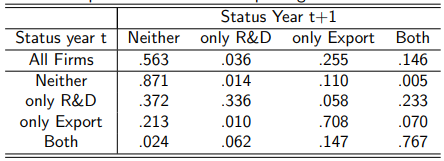
\includegraphics[width=0.7\linewidth]{screenshot002}
	\caption{Матрица перехода для решений инвестировать в НИОКР и экспортировать }
	\label{fig:screenshot002}
\end{figure}



\end{frame}




\section{Оценка модели}




\begin{frame}[shrink=3]
\frametitle{\insertsection} 

\begin{figure}
	\centering
	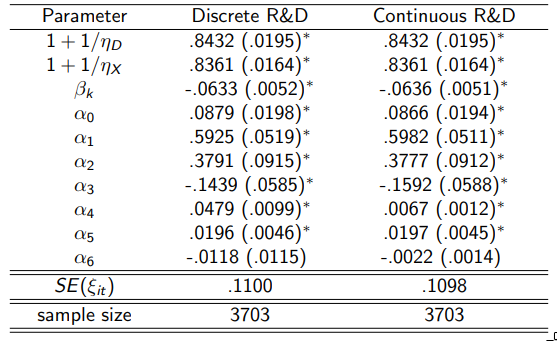
\includegraphics[width=0.7\linewidth]{screenshot010}
	\caption{Оценки динамики производительности}
	\label{fig:screenshot010}
\end{figure}


\begin{figure}
	\centering
	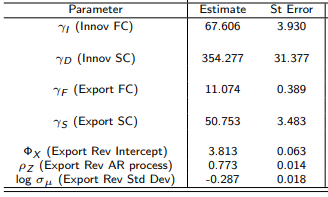
\includegraphics[width=0.7\linewidth]{screenshot011}
	\caption{Оценки динамики принятия решений}
	\label{fig:screenshot011}
\end{figure}


\end{frame}


\begin{frame}[shrink=3]
\frametitle{\insertsection} 


\begin{figure}
	\centering
	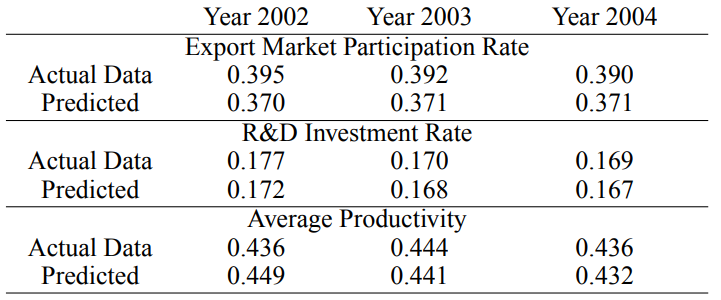
\includegraphics[width=0.7\linewidth]{screenshot012}
	\caption{Прогноз уровней производительности, вовлеченности в инвестирование и экспорт}
	\label{fig:screenshot012}
\end{figure}

\begin{figure}
	\centering
	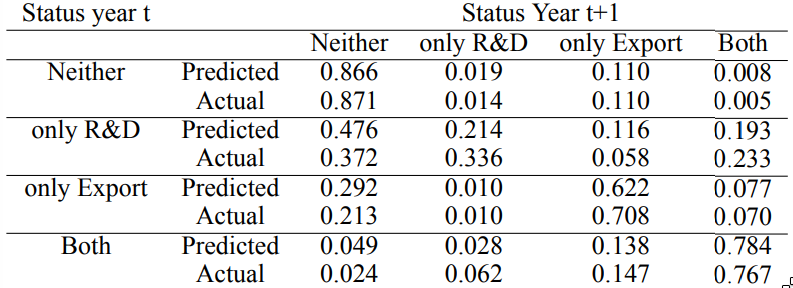
\includegraphics[width=0.7\linewidth]{screenshot013}
	\caption{Прогноз матрицы перехода для фирм, продолжающих свою деятельность }
	\label{fig:screenshot013}
\end{figure}


\end{frame}


\section{Результат}




\begin{frame}[shrink=3]
\frametitle{\insertsection} 


Динамика производительности (оценка  $g(·)$):

$$\dfrac{ \Delta x_{it}>0}{\Delta e_{it-1}} > 0; \dfrac{\Delta x_{it}}{\Delta d_{it−1}}> 0; \dfrac{\Delta^2x_{it}}{\Delta e_{it}\Delta d_{it}}< 0$$



\begin{itemize}
	\item Производительность растет в ответ на НИОКР и экспорт.
	\item Воздействие НИОКР на производительность больше,  но относительно низкая стоимость экспорта делает его более популярным выбором.

\end{itemize}


Невозвратные  и постоянные затраты на экспорт и НИОКР:

\begin{itemize}
\item  Расходы на НИОКР примерно вдвое больше, чем расходы на экспорт 
\item  Невозвратные издержки  примерно в два раза больше фиксированных 
\item  Составляют около 10\% доходов
\end{itemize}

Взаимозависимость между экспортом и инвестициями в НИОКР:
\begin{itemize}
\item  "Отбор" основанный на производительности фирмы $x_{it}$ для  $e_{it}$ и $d_{it}$ (с учетом стабильного экспортного спроса)
\item   Постоянства в выборе из-за больших по сравнению с фиксированными издержками  невозвратных расходов
\item Вероятность экспортировать уменьшается при инвестировании  в НИОКР и вероятность
инвестировать  в НИОКР уменьшаются при экспорте

\end{itemize}






\end{frame}



\end{document}